\chapter{Low-fidelity prototyp}

\todo[inline, color=blue!30]{UPDATE: Postupně přidávám další kapitoly. Není dokončené, zatím v procesu.}

\todo[inline, color=blue!30]{Do téhle kapitoly by se ještě mělo vejít porovnání různých nástrojů a proč jsme se tak rozhodli.}

Po storyboardech, které nám ukázali možné sekvence akcí, vytvoříme prototyp aplikace, se kterým budou interagovat uživatelé. V rámci ročníkového projektu vytvoříme jen low-fidelity prototyp. Tedy se budeme zabývat vytvořením rané verze aplikace, která nebude věrnou kopií aplikace výsledné. V této fázi, chceme hlavně rychle vytvořit prototyp, na kterém můžeme vyhodnocovat nápady a zároveň ho můžeme otestovat na uživatelích spadajících do jednotlivých uživatelských skupin, které jsme si definovali.

\section{Paper prototyping}

Pro navrhování a testování uživatelského rozhraní ve verzi low-fidelity jsme si vybrali jednu z využívaných metod, prototypování na papír (paper prototyping). Celý proces od vytvoření prototypu až po uživatelské testování popisuje detailně kniha Paper prototyping od Carolyn Snyder \cite{Paper_Prototyping}.

Začneme vytvořením papírových komponent aplikace (oken, menu, stránek, dialogových boxů, dat, pop-up zpráv). 
Po vytvoření prototypu provedeme usability otestování.
V takovém testování provádí uživatel, v jednom sezení, realistické úkoly na papírovém prototypu. Nejedná se o studii, kdy jsou prováděny série testů použitelnosti během několika dní. Uživatelé jsou vybraní podle uživatelských skupin, které jsme si definovali na začátku.

Prototyp bude ovládaný osobou, která reprezentuje konání počítače, ale nevysvětluje, jak má rozhraní fungovat. Další zkušený člověk funguje jako zapisující pozorovatel. Pozoruje chování uživatele, zapisuje co uživatel dělá a co říká. Tímto způsobem provedeme velmi rychle iterativní testování na několika uživatelích. V průběhu můžeme aplikaci vylepšovat a všímat si opakujících se vzorů. Každé sezení s uživatelem končí vyplněním dotazníku spokojenosti s aplikací.

\subsection{Vytváření prototypu}

Papírový prototyp vytvoříme v nezávislosti na existujících aplikacích. V tomto momentě je dobré si ujasnit, na jakém zařízení budeme aplikaci používat. Tak nějak implicitně jsme od začátku předpokládali, že půjde o počítačové rozhraní. Mobilní aplikace se k němu nepřidá, alespoň ne ve verzi s možností úprav. Stejně tak aplikace pro tablety. Tahle zařízení jsou užší a menší. Mají tak méně prostoru pro obsah, navigaci a interakci. Použití modelovacích a složitějších funkčností by tak bylo často složité až nemožné.

Jako inspirace nám posloužili existující webové nástroje a desktopové aplikace.  ... Railway aplikace, Draw.io (hlavně u ER modelování ta obrazovka vlevo)   ... Díky konzistenci v aplikaci uživatelé v posledním úkolu nebyli špatní 

V mockupu popsat jednotlivé komponenty a napsat k nim, tady jsme se inspirovali tím a tím,

Zaměřili jsme se na to, jestli jsou komponenty dostupné, jestli nic nemate uživatele, když má na něco kliknout...

Když se má uživatel někam dostat, tak aby ho nerozptylovaly komponenty a věděl na co chce kliknout

nesnažíme se z toho dělat vyloženě závěry, jenom se snažíme poukázat na podobnosti s návrhem person

Rozložení: F-Pattern, kam se dostanu po kolika kliknutích, F-Pattern se nehodí pro telefony, je dobré F-Pattern použít jako základ, ale vyloženě se tím neřídit (dnes spíš tíhne k rozmanitosti), The F-Pattern is mirrored in right-to-left languages, such as Arabic, aplikace psaná anglicky -> jsme zvyklí číst zleva doprava

\begin{figure}[htb]
    \centering
    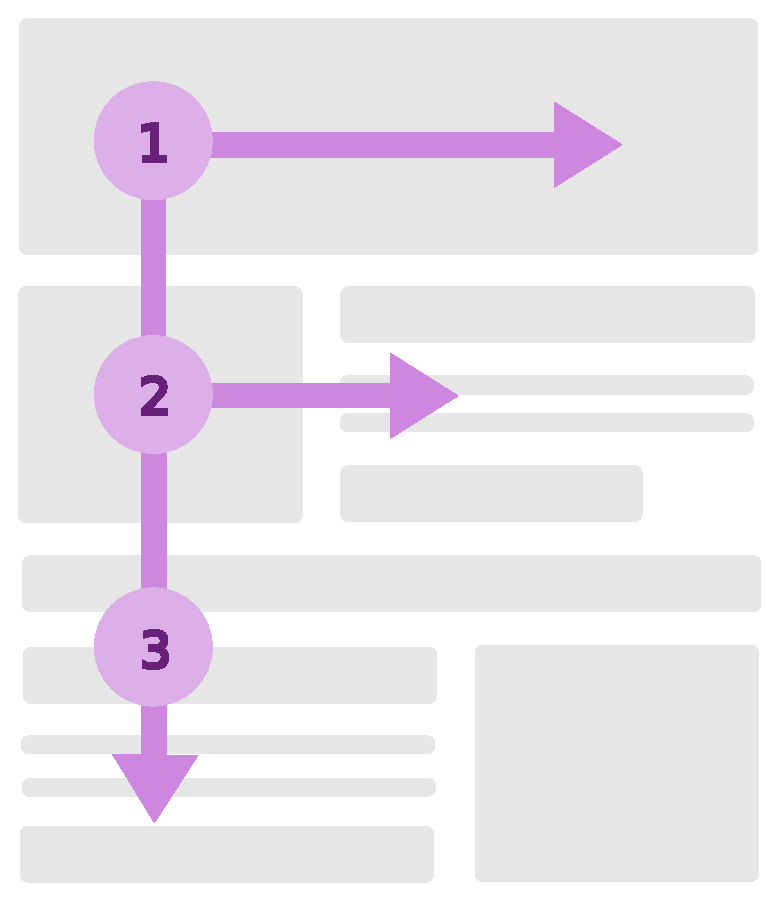
\includegraphics[height=70mm]{../img/F-Pattern}
    \caption{F-Pattern layout.}
    \label{obr03:fpattern}
  \end{figure}

Subsekce na:
- existující nástroje, kterýma jsme se inspirovali (Ukázat několik aplikací a porovnat, proč jsme se rozhodli tak a tak to udělat (jedna z nich https://app.sqldbm.com/PostgreSQL/DatabaseExplorer/Draft/).)
- konkrétní návrh -> popsání hlavní obrazovky, zaměření se na plovoucí komponenty

\section{Uživatelské testování}

Proč vůbec chceme low-fidelity návrh testovat na uživatelích? Kromě toho, že papírový návrh se dá rychle měnit, se můžeme vyhnout hnidopišské zpětné vazbě. O ní se zmiňují i v knize Paper Prototyping na straně 58 \cite{Paper_Prototyping}. Komponenty a barvy nejsou jasně dané, uživatel se spíš zaměří na koncepty a funkčnost. Je totiž očividné, že jsme ještě nespecifikovali vzhled. Schumann a další se v jednom ze svých článků \cite{Schumann_1996_AEN} zabývají tím, že nedokončený návrh povzbuzuje ke kreativitě a k tomu, aby uživatel nebyl pasivní a sám přemýšlel nad koncepty. 

Připravíme si úkoly, které budou uživatelé dělat. Budou to ty nejběžnější, které jsme rozebírali v předchozích kapitolách. Jmenovitě první úkol, kdy uživatel přidá databázovou komponentu. Další hlavní úkol je vytvoření jednoduchého schématu a~poslední jeho dekompozice.
Po připravení úkolů najdeme uživatele spadající do vytvořených uživatelských skupin. Dáváme si pozor, aby neznali aplikaci nebo naše názory na ni.

V kapitole Some Techniques for Observing Users knihy The Art of Human-computer Interface Design \cite{Brenda_1990_art} autorka popisuje techniky pro pozorování uživatelů, které se nám při testování budou hodit. Chceme zjistit, kde mají uživatelé problém aplikaci používat a co jim naopak vyhovuje.

Pro samotné testování vybereme místo, které je tiché a bez zbytečných vnějších vyrušování. Popíšeme uživateli o co se jedná a vyvětlíme, že jsou zapojeni do raných fází návrhu. Zdůrazníme, že testujeme aplikaci, ne uživatele. Poprosíme uživatele, aby přemýšleli nahlas a říkali to co jim přijde na mysl v průběhu plnění úkolů. Díky tomu prozkoumáme jejich očekávání od produktu, taky jejich úmysly a jejich strategie řešení problémů. Nakonec ještě upozorníme, že nebudeme uživateli pomáhat při plnění úkolů. Je to nejlepší způsob jak zjistit jak uživatelé reálně interagují s aplikací.

Po otestování zodpovíme zbývající otázky od uživatele. Případně diskutujeme nějaké zajímavé chování, které uživatel při testování měl. Závěrem pak bude vyplnění dotazníku uživatelem. Je důležité, aby v dotazníku byly jenom otevřené otázky, které uživatele nijak nenavádí. Ptáme se hlavně na pocity z aplikace, jestli něco neodvádělo pozornost uživatele a jestli dává smysl navigace po aplikaci.

\section{Závěr z uživatelského testování}

\todo{Do téhle podkapitoly dát obrázek z průběhu uživatelského testování}

Pro otestování jsme získali tolik a tolik uživatelů.

mám 2 zdroje, dotazník a zápisky z testování...
